%% This is an example first chapter.  You should put chapter/appendix that you
%% write into a separate file, and add a line \include{yourfilename} to
%% main.tex, where `yourfilename.tex' is the name of the chapter/appendix file.
%% You can process specific files by typing their names in at the 
%% \files=
%% prompt when you run the file main.tex through LaTeX.

fix the abstract to include UPC (currently only FIB is shown)
\nocite{Stefanov} \nocite{Crockford} \nocite{Darwin} \nocite{AngularJSGuide} 

\chapter{Introduction}
% possible quotations: welcome humans. goodwill. and we have a plan.
This is a report for a master's thesis.
This document is a stand alone presentation of the work done, which belongs to a larger project: the Content Management System (codenamed \textit{Flango}) for the robots.
More specifically, this thesis deals with the reengineering of Flango \cm , the part of the system deployed in the robot that renders the screens on the touchscreen, with web technology.
Using web technology in a component of the robot is a novelty in the company.
It is desired not only to develop a practical solution but also to guarantee that the final output of the Flango \cm is the same that the old system generates.

This thesis is eminently a practical work, although the theoretical background has been extensively explored. 
It is done to develop a sustainable product based on open standards (as opposed to the current implementation with \flash) that can be extended and reused for other robotic products that might be designed in the future.

\section{\company}
\company is a company based in Barcelona dedicated to R\&D of humanoid robots and robotic components. 
An international team of mostly mechanical, electronics and software engineers pushes forward the research on different fields, like speech recognition and generation, computer vision, walking, grasping, machine learning and navigation amongst others.
The company has developed 5 humanoid robots until 2013: \reem{A}, \reem{B}, \reem{H1}, H2 and H3, and \reem{C}.
This project targets \reem{H2} and H3, service robots with wheels.

\subsection{Reem H2 and H3}
\reem{H2} \fref{fig:reemh2} and H3 \fref{fig:reemh3} are humanoid service robots featuring a screen on their torso.
They have an autonomous navigation system, speech recognition and voice synthesiser, they can find their way in different settings and help or entertain people in a friendly way.
They are intended for use in public places such as hotels, malls, airports or museums.

\begin{figure}
   \centering
   \begin{subfigure}[b]{0.4\linewidth}
       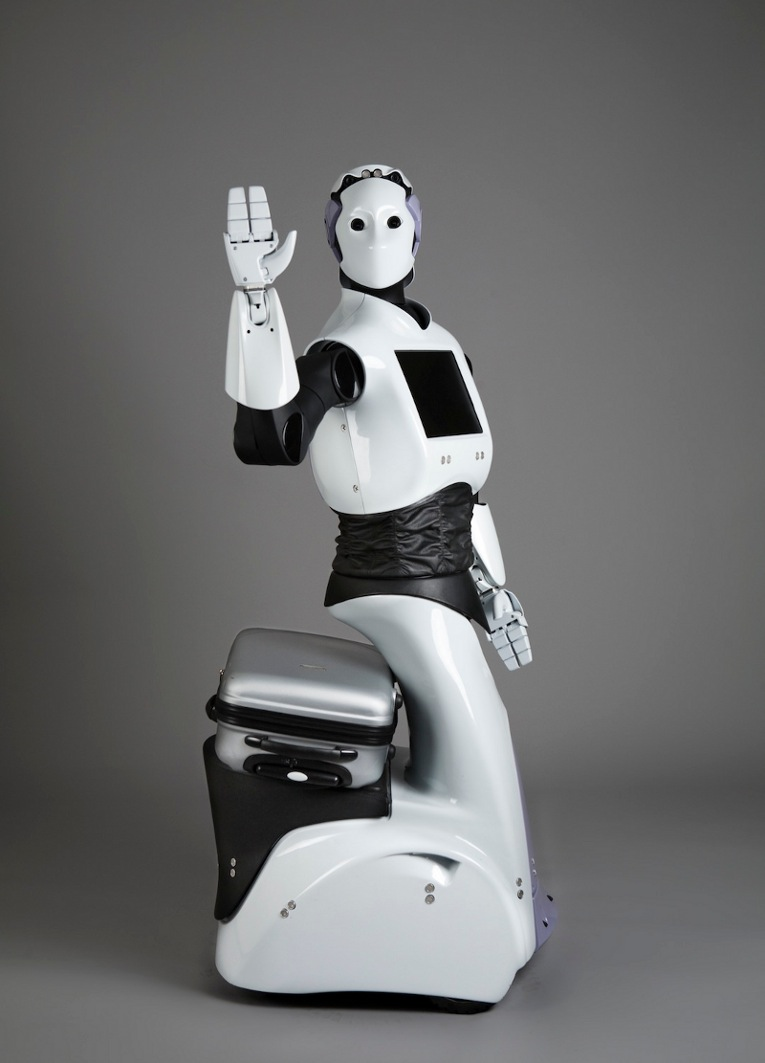
\includegraphics{figures/reemh2}
       \caption{\reem{H2}}
       \label{fig:reemh2}
    \end{subfigure}
    \begin{subfigure}[b]{0.4\linewidth}
           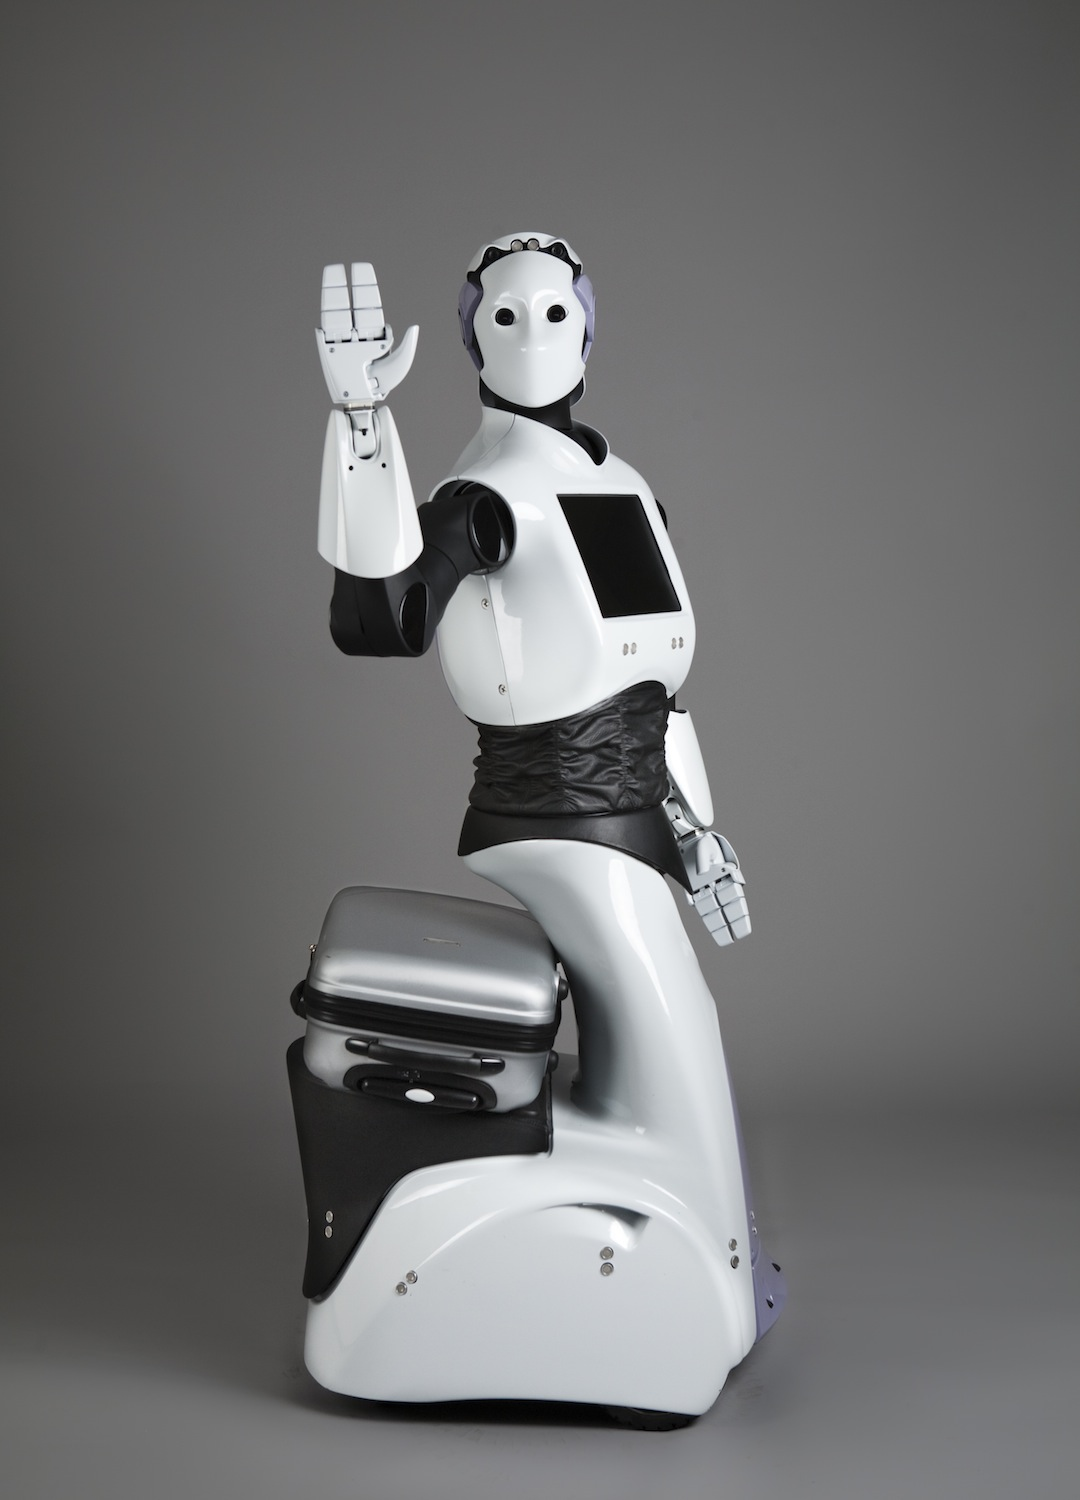
\includegraphics{figures/reemh3}
           \caption{\reem{H3}}
           \label{fig:reemh3}
    \end{subfigure}
    \caption{\reem{H} Series}
    \label{fig:reemseries}
\end{figure}

\begin{table}[ht]
    \centering
    \begin{tabularx}{\linewidth}{| X | X | X |}
    \hline
    Weight & 90 Kg & x same\\ \hline
    Height & 1.70 m & same \\ \hline
    Battery life & 8 h & same \\ \hline
    Degrees of freedom & 22 & same \\ \hline
    Payload & 30 Kg (mobile base), 3 Kg/arm & same\\ \hline
    Speed & 4 Km/h & same\\ \hline
    Computer & Core 2 Duo + Atom & Core 2 Duo + Atom \\ \hline
    Sensors & Microphone, stereo-camera, laser, ultrasounds, accelerometers and gyroscopes & same \\
    \hline
    \end{tabularx}
    \caption{Reem H2 and H3}
    \label{tab:rh2}
\end{table}

\section{The Current System}
The \reem{H} series have big potential in human robot interaction. 
These humanoid robots have a multi-modal interface: besides speech or joystick manual control, humans can use a touch screen to command the robot or obtain information.
\reem{H} can display multimedia contents like corporate videos, information about the client, capabilities of the robot, language settings, etc.

\begin{figure}[htb]
    
    \centering
    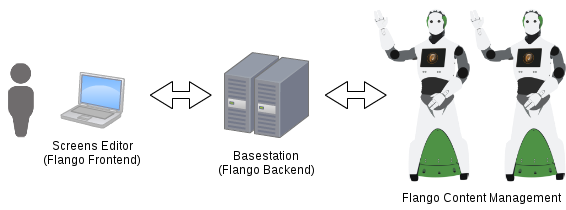
\includegraphics[width=14cm]{figures/intro-system-overview}
    \caption{Overview of the system}
    \label{fig:intro-system-overview}
\end{figure}

The Contents Management System comprises \emph{\flangofe} and \emph{\flangobe} (both in Basestation), and \emph{Flango \cm} (in the robot).
The Basestation is an application server that hosts Flango, a \ac{RIA} to manage contents and robots made with Django, a widely used framework for Python. 
Clients can create contents applications  with the \flangofe (\se), a tool built with \flash .
When application contents are ready, clients can associate $1$ application with $n$ robots to display it in the touch screen.

\lstinputlisting[label=example-screen-xml,language=XML, caption={Example Screen XML}, breaklines=true]{src/example-screen.xml}

The elements of a contents application (screens and entities) have an \ac{XML} representation (\ref{example-screen-xml}), an approach similar to popular projects (e.g. Android, NetBeans) and even, in a sense, all \acp{RIA} made with \ac{HTML}.

A contents application is essentially a set of screens, navigation multimedia contents that users can manage with the media library, and entities. 
FIXME LANGUAGE The last are domain objects that can be instantiated and represented in a view. 
This way a client can create an application that shows information about the company, include buttons to provide an easy way to give commands to the robot (e.g. "follow me", "shake hands"), display videos and picture galleries, etc.
All of these components are localisable. 
They can be resized, repositioned, repainted... depending on the current language.
This allows for more human-robot interaction and enriches the experience. 
Using other tools, clients can also associate sentences to screens and the speech synthesiser reads them aloud.

\begin{figure}[htb]
    \label{fig:screens-editor}
    \centering
    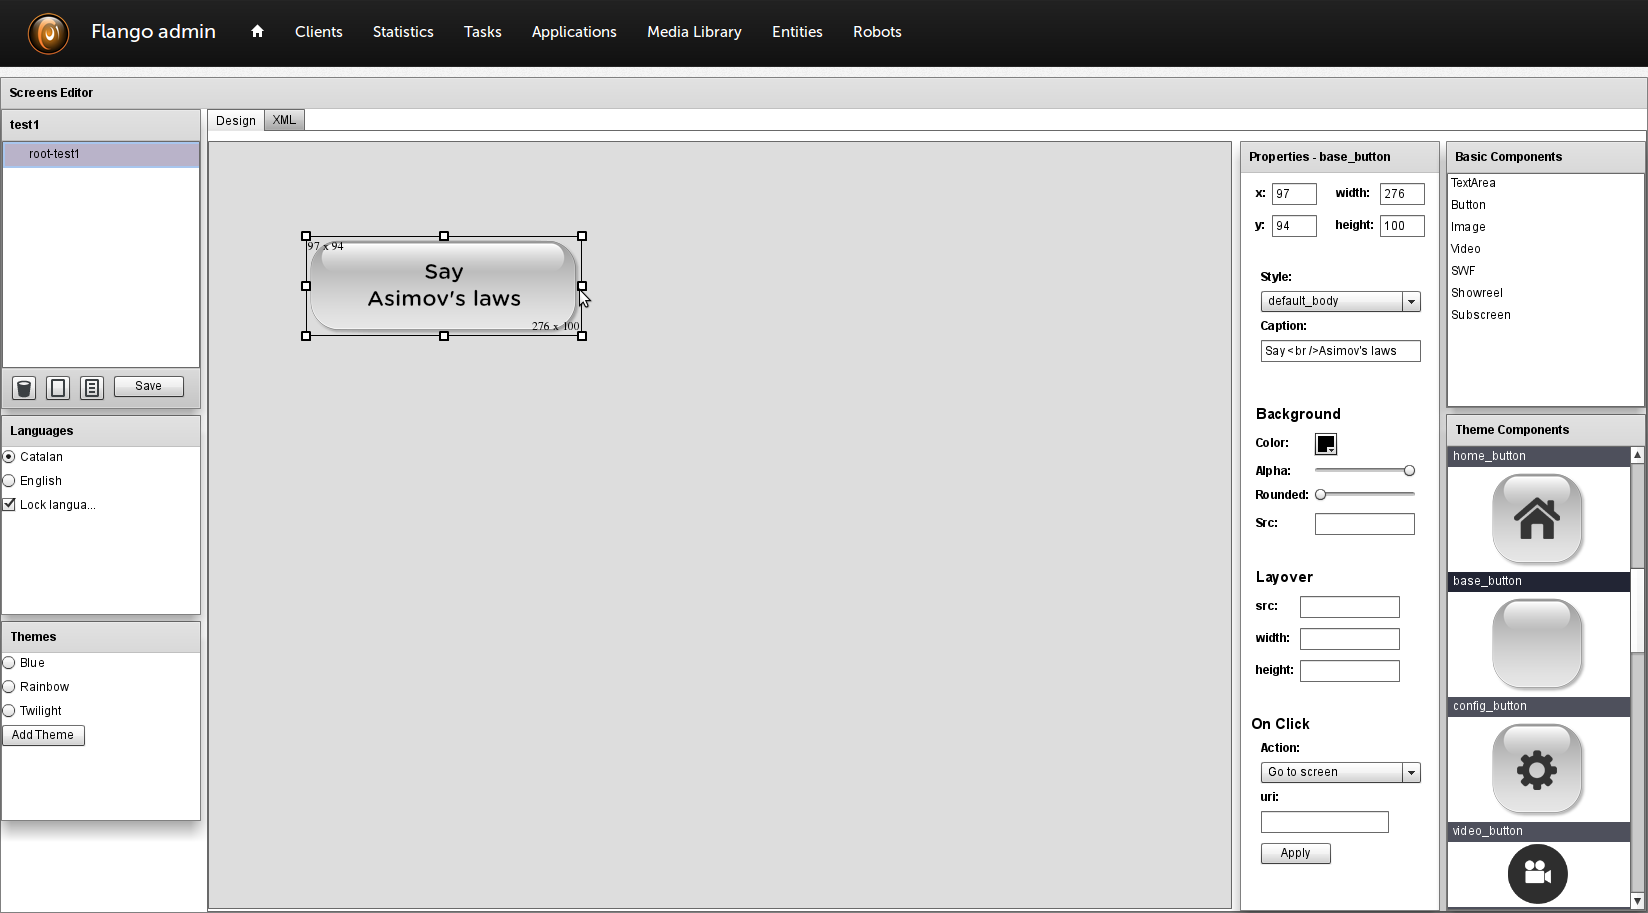
\includegraphics[width=\textwidth]{figures/screens-editor}
    \caption{Screens Editor, a Flash application in Flango}
\end{figure}

\reem{} robots have a built-in software to render the content applications. 
It is also made with \flash .
The main responsibility of this software is transforming \ac{XML} files into a \ac{UI}. 
Initially, this software has no \ac{GUI} or direct interaction with a person.

\begin{figure}[htb]
    \label{fig:xml-flango-view}
    \centering
    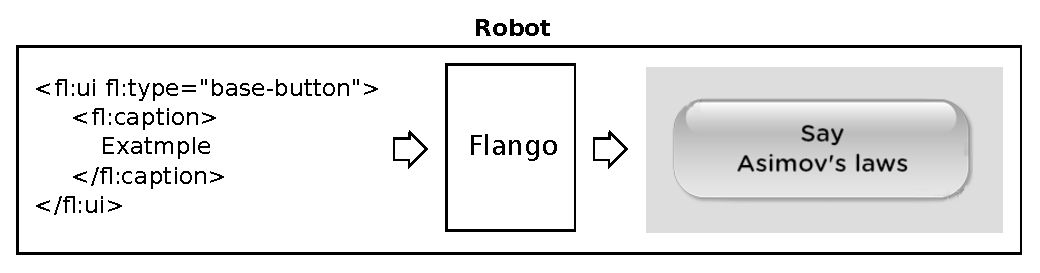
\includegraphics[width=\textwidth]{figures/xml-flango-screenshot}
    \caption{From \ac{XML} to the \ac{GUI}}
\end{figure}

This thesis documents the project to \textbf{re-engineer the \cm , in the robot, to use modern web technologies instead of \flash}.

\section{The New System}
The \ac{WWW} was born as a document viewing platform and has evolved gradually into an application platform. 
First the web consisted of simple pages that contained structured text and some images. 
Navigation was done using simple links between pages. 
In a second phase, web sites became interactive: 
it was the time of animated graphics, browser plug-ins and JavaScript. 
More recently web sites have adopted features from traditional desktop software in \acp{RIA} \cite{Anttonen:2011}.

For a decade, the \flash player plug-in has provided a platform to enable rich and interactive content in browsers.
However, Adobe has made the updates exclusive to the Google Chrome\textsuperscript{\textcopyright}\xspace browser \cite{FlashRoadmap}. 
The browser in the robot application, QtWebBrowser, uses this plug-in but will not receive updates from Adobe and \company systems need to adapt to this new setting. 
There are two solutions:
\begin{itemize}
	\item Use Google Chrome instead of QtWebKit
	\item Use modern web technologies, either in QtWebKit or in another browser
\end{itemize}

The solution is rethinking the application to be a part of the robot's system and implement it with modern web technology.
There is a number of technologies that could be used but the web allows the product to be easily portable, very extensible, open to many developers and sustainable as it does not depend on a single company.
\ac{HTML5} is perhaps the best known forthcoming standard in the Web and is typically combined with JavaScript and \ac{CSS3}. 
It has become such a popular combination that major browser vendors provide support for the latest drafts of the \ac{W3C}, like the audio \ac{API} for \ac{HTML5} or the video support.
A big number of frameworks with JavaScript have appeared not only client-side (e.g. BackBone, jQuery, Ext JS, Google Web Toolkit, Yahoo User Interface Library...), but even server-side (e.g. NodeJS).
Moreover, new \ac{HTML5} capabilities and \acp{API} are an opportunity to add features to this project.

The project of this thesis uses Google AngularJS\copyright, a \ac{MVC} framework that lets developers \emph{teach the browser new syntax}. 
Thus, the syntax of the \ac{XML} files coming from the \se can be interpreted natively in a browser. 
This has some advantages over \flash \cite{Jobs:ThoughtsOnFlash}:
\begin{itemize}
    \item No use of third-party plug-ins
    \item Openness
    \item Reliability, security and performance
    \item Keeps power consumption lower (e.g. using the GPU to decode video or apply transformations and smooth transitions to elements on the screen)
    \item Touch-enabled: the new screen of Reem H3 is multi-touch. To enable gestures, heavy rewriting of the current Flash application is required.
\end{itemize}

%\section{Context of the work}
%TODO FIXME

%The work context diagram identifies the boundaries of the work that you need to investigate to be able to build the product. Note that it includes more than the intended product. Unless we understand the work that the product will support, we have little chance of building a product that will fit cleanly into its environment.

%The adjacent systems on the context diagram (e.g., Weather Forecasting Service) indicate other subject matter domains (systems, people, and organizations) that need to be understood. The interfaces between the adjacent systems and the work context indicate why we are interested in the adjacent system. In the case of Weather Forecasting Service, we can say that we are interested in the details of when, how, where, who, what, and why it produces the District Weather Forecasts information.

%motivation To clearly define the boundary for the study of the work and hence the requirements effort. Without this definition, we have little chance of building a product that will fit seamlessly into its environment


\section{Goals}
TODO: This section should probably be expanded

This thesis is part of the specialisation of Software Engineering and Information Systems. 
The goal is to reengineer the Flango \cm with web technology.
More specifically, the author has to gather the requirements from an existing system, plan in terms of scope, time and cost, make the system specifications, design and implement it using modern web technologies, use quality assurance tools and deploy it successfully in a \reem{H3} robot.

Regarding the project, the goals are:
\begin{itemize}
	\item Reengineer the current system with web technology
	\item Develop a testing strategy to make it robust
	\item Make it compatible with non-reengineered parts of the system
\end{itemize}


\section{Organisation of this document}
This document describes the system developed at \company to render the screens created with the \se on the \reem{H2} and H3 series.
It does not cover other software on the robots or in Basestation.

% TODO check the easy to read phrase
This project has been developed iteratively using a \ac{TDD} methodology. 
This document presents the system in a chronological manner as if it had followed the classical software life cycle in its development, hoping to offer an easier reading:
It first analyses the state of the art and includes some background knowledge required to understand the decisions taken during the development, then the planning and the requirements, the specification of the system, the internal design (with special attention to the framework and the specific technology of both the hardware and the software), some examples of the implementation and the testing strategy.
Readers will find an overview section at the beginning of each chapter to put them in context.

This document describes the project as follows:
\begin{description}
\item[Related Work] Provides a general overview of topics surrounding those of this thesis, enabling for a deeper understanding of the material at hand.
It starts with a description of the reengineering process, followed by a section about web technology and finally, a description of the methodology of the project (\ac{TDD}).

\item[Project Management] Contains information about the project from the point of view of management. 
Detailing on schedule, budget and risk analisys. Contains an assesment of the execution.

\item[Requirements] States the functional and non-functional minimum requirements, the constraints and and weights the use of off-the-shelf solutions.

\item[Specification] Defines what the application does in the context of a reengineering process. 
It offers the first three steps: a software inventory, [documentation restructuring] and a description of the current system (with special attention to context, interoperability and interaction).
Contains the specification of the new system: a conceptual model, use cases and the behaviour model, with sequence diagrams and contracts of system operations. 

\item[Design] Describes the internal design of the software in the context of a reengineering process. 
It contains the last three steps: code restructuring, data restructuring and forward engineering.
Detailing about the system architecture and the context and the patterns used.
Contains a static view (class and packages diagram), a dynamic view (sequence diagrams) with examples of the most relevant operations and a physical view (deployment diagrams)

\item[Implementation] Holds technical details about the environment, the set-up, the integration in the robot and a larger system and meaningful examples of the technology used. 
Emphasises the implementation of the patterns described in previous chapters.

\item[Testing] Describes the implementation of the testing strategy, the goals and the integration in the robot system.

\item[Conclusion] Presents the conclusions from technical, academic and personal point of view. 
Includes challenges faced during developments and future work. FIXME


\item[Appendix A] Lists unit tests that define the behaviour of most components of this system.

\end{description}